% A skeleton file for producing Computer Engineering reports
% https://kgcoe-git.rit.edu/jgm6496/KGCOEReport_template

\documentclass[CMPE]{KGCOEReport}

% The following should be changed to represent your personal information
\newcommand{\classCode}{CMPE 663}  % 4 char code with number
\newcommand{\name}{Andrei Tumbar}
\newcommand{\LabSectionNum}{1}
\newcommand{\LabInstructor}{Wolfe}
\newcommand{\TAs}{Nitin Borhade}
\newcommand{\exerciseNumber}{2}
\newcommand{\exerciseDescription}{Servos}

\usepackage{tikz}
\usepackage{circuitikz}
\usetikzlibrary{calc}
\usepackage{multirow}
\usepackage{titlesec}
\usepackage{float}
\usepackage{lmodern}
\usepackage{siunitx}
\usepackage{subcaption}
\usepackage{graphicx}
\usepackage[usestackEOL]{stackengine}
\usepackage{scalerel}
\usepackage[T1]{fontenc}
\usepackage{amsmath}


\def\code#1{\texttt{#1}}

\begin{document}
    \maketitle
    \section*{Analysis/Design}

    This project looked at implementing a motor controller that could take
    user input as well as run a predefined set of instructions. Instructions
    were encoded into a single byte with the first three bits acting as an
    op-code and the final five bits as a a parameter. The design of the entire
    system was split into multiple independent modules. An executor was created
    for executing task modules at various rates. A table of tasks can be found
    in \code{main()} called \code{task\_table[]}. \\
    
    \begin{figure}[h!]
      \centering
      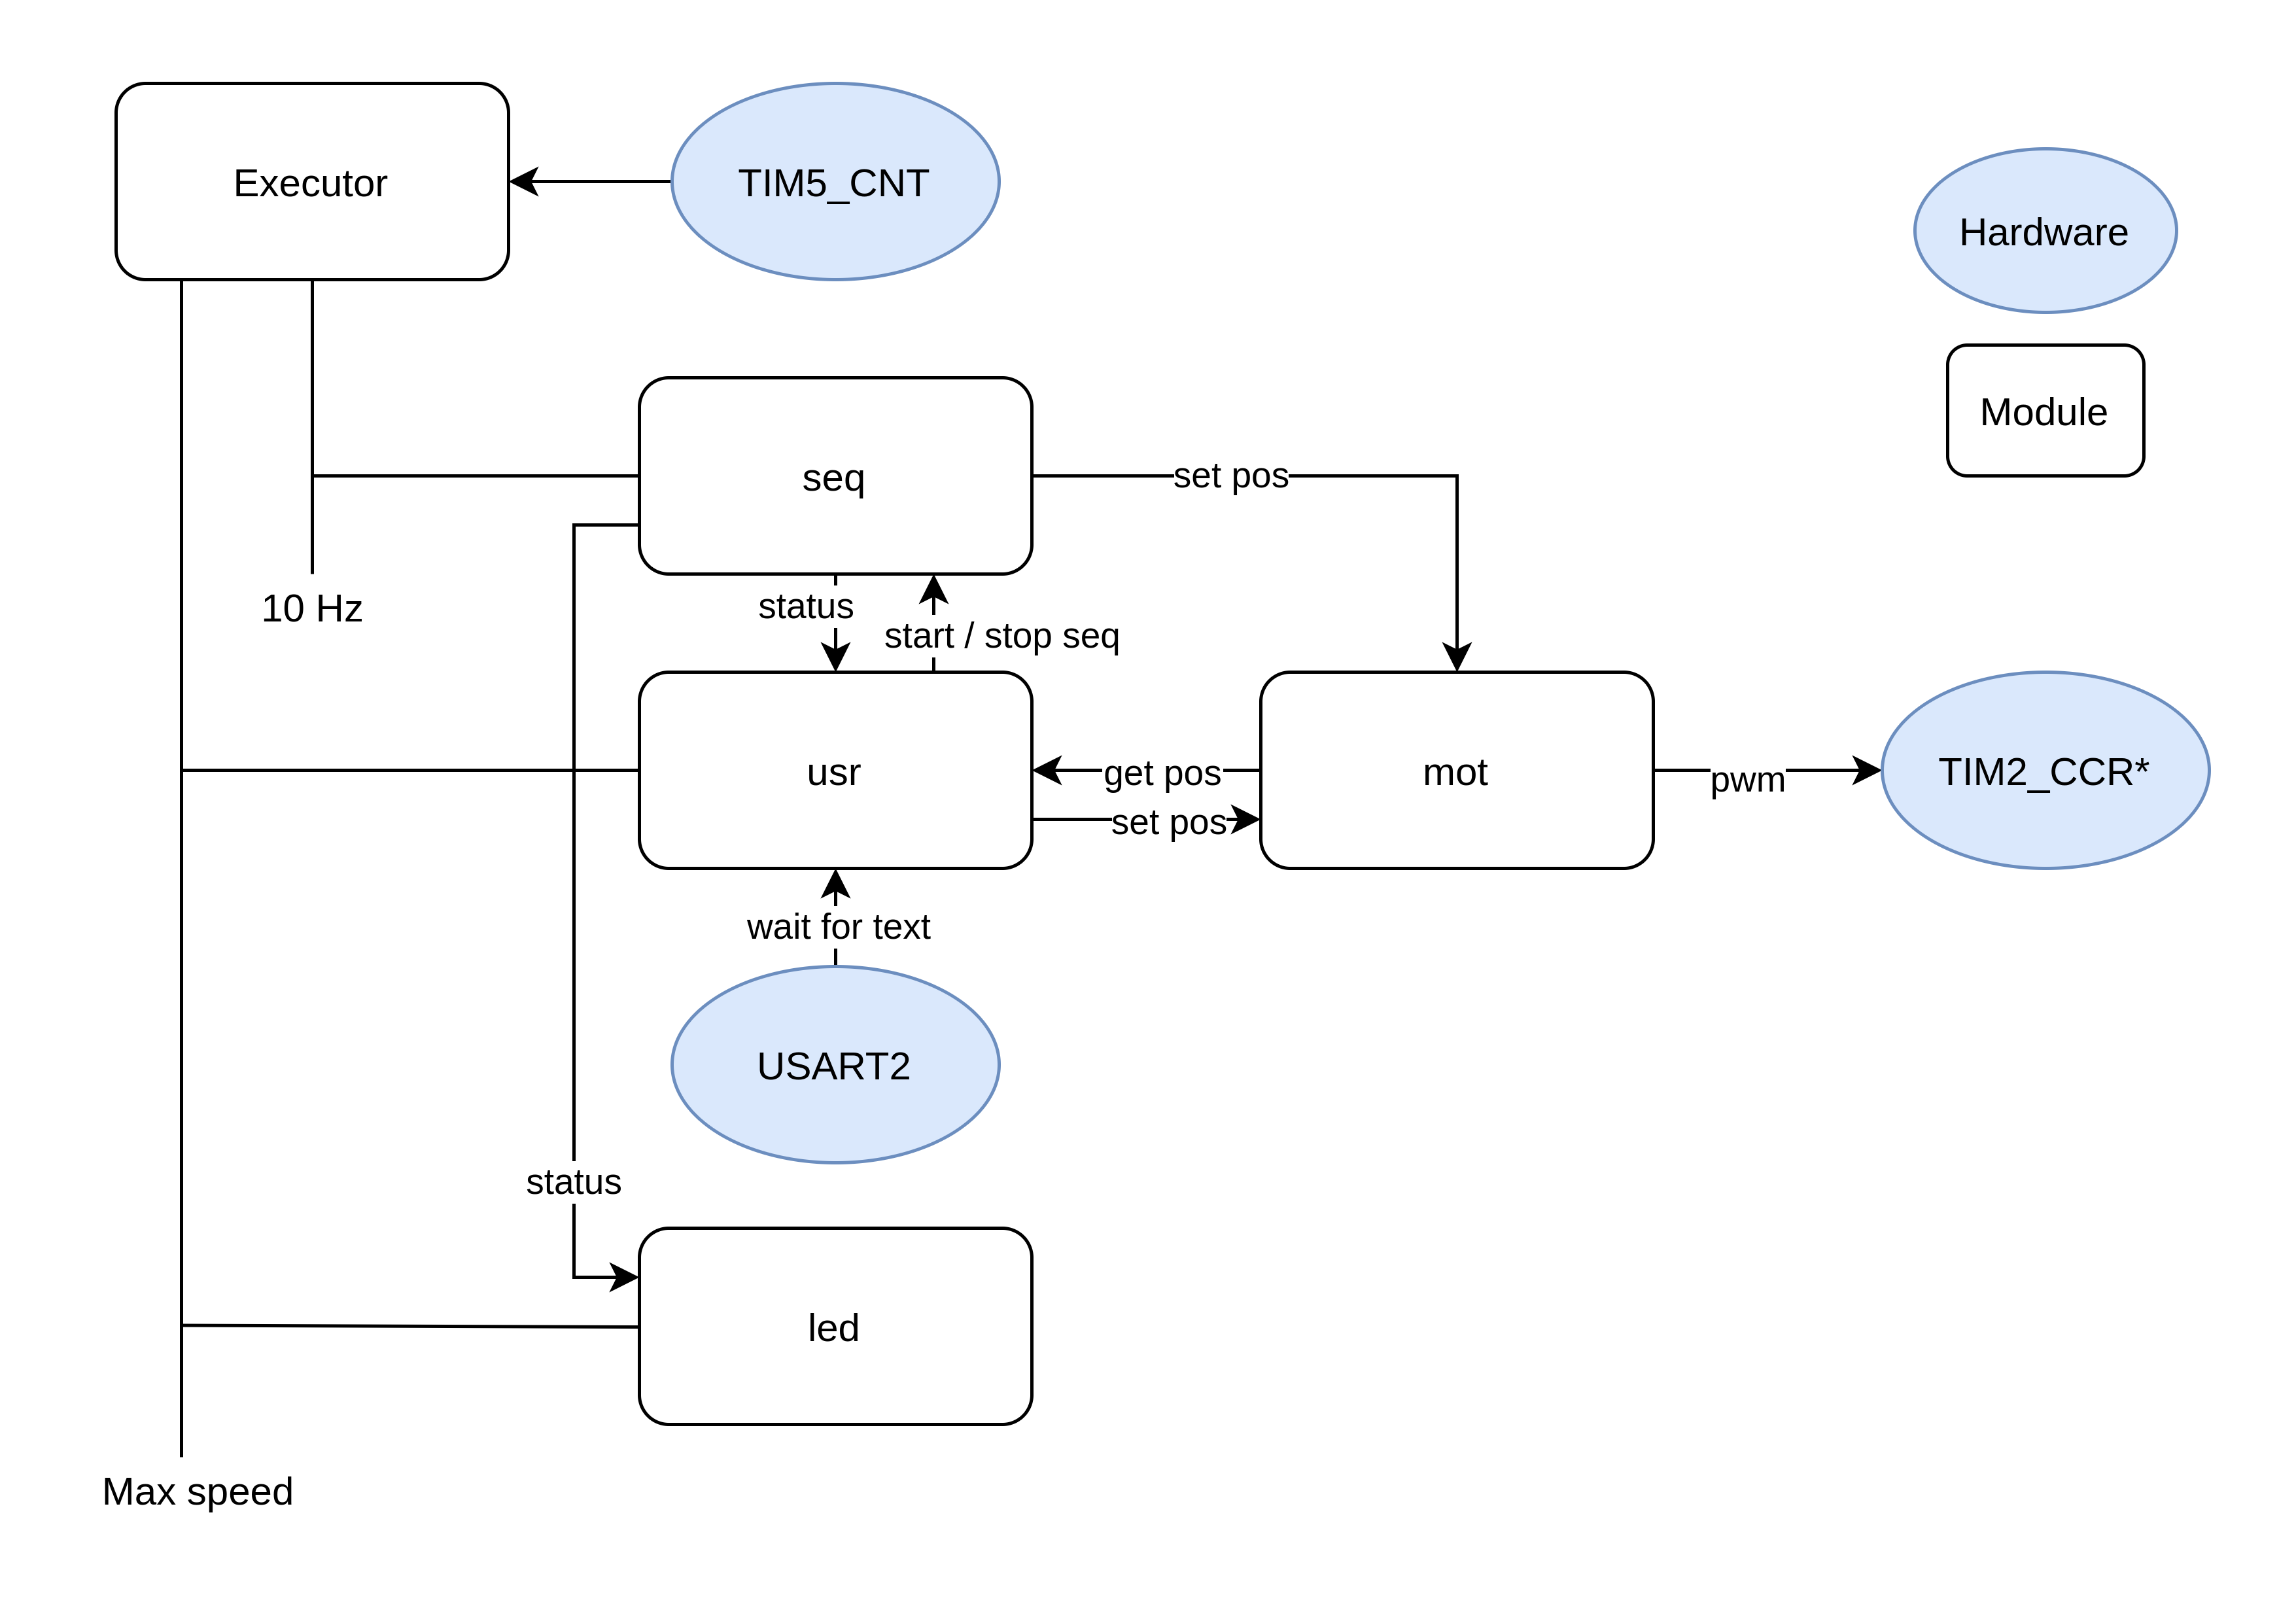
\includegraphics[width=5.5in]{servo_proj_design}
      \caption{Design of servo control project}
      \label{fig:overview}
    \end{figure}
    
    The first and most
    important module is \code{mot} (Motor). This module is responsible for
    keeping track of motor position and providing a public interface for
    getting and setting motor position. This module utilized a PWM conversion
    table to produce a correct duty-cycle given a target position.\\

    \code{seq} (Sequence or recipe) is responsible for keeping state of an
    executing recipe on the specified motor. Two sequence engines were
    instantiated pointing to either servo motors. The implementation involved
    a program counter and instruction table to decode from.
    Each opcode would then dispatch a separate function and could interface
    with \code{mot} if needed. Because the \code{seq} module was implemented
    as a task (as opposed to \code{mot} which is a service), it has a executor
    interface that is expected to be called at 10 Hz.\\

	Finally, \code{usr} and \code{led} are also implemented as tasks, however
	their execution are not delayed by a hardware timer. Their non-blocking
	task will be executed at the maximum speed the software can attain. \code{led}
	simply looks at the status code of both sequence engines and controls four
	LEDs to denote each of the four states per motor. \code{usr} will take input
	from the user and control \code{seq} and \code{mot} as needed.

	\subsection*{Grad-portion}

	For the grad-portion of the assignment, an extra op-code was implemented
	called \code{ERROR\_IF}. This opcode would check the position of the opposite
	motor and cause recipe failure if the motor was at a given position. For
	example, if \code{ERROR\_IF|3} was running on motor \code{1} and motor
	\code{2} was at position \code{3}, the recipe on motor \code{1} would fault
	out. To easily test this behaviour, an extra set of user command was
	implemented, any ascii character from \code{'0'} to \code{'5'} could directly
	set the position of the motor in question.

    \section*{Test Plan}

    Testing the code was fairly straighforward. I started by implementing
   	\code{mot} and testing each motor position on either motor. Once this
   	was working, I wrote the \code{seq} state machine and made sure the timing
   	provided by \code{TIM5} was accurate. The extra set of user commands
   	discussed in the grad-portion section of this document also proved very
   	useful for the testing of \code{usr}, \code{seq} and \code{mot}.

    \section*{Project Results}

    The software behaved as expected by the problem statement. Motor 1's
    recipe \code{MOV} commands as well as the \code{WAIT} commands produced
    the expected delays of $9.3s + 0.2 \cdot \delta_{position}$. User input
    could be gathered at any point during program execution including during
    the execution of a recipe. This was done by writing all tasks as a
    non-blocking interface so as to allow the execution of all tasks.

    \section*{Lessons Learned}

	This project explored creating an embedded system with multiple simultaneous
	cooperating tasks running. It also tought me how servo motors are controlled
	with a PWM signal. While the hardware component of this project was fairly
	straightforward, the software was written to be robust enough to fault
	execution if invalid branches or parameters were seen. This caught several
	bugs and sped for project up considerably.

\end{document}
